\section{Theory}
\label{sec:Theory}
\subsection{The Sagnac Interferometer}
\label{sec:The_Sagnac_Interferometer}
A Sagnac interferometer is a device built out of multiple mirrors and a polarising beam splitter cube (PBSC). Its purpose is to split a laser beam entering the interferometer into two beams, which can then be redirected over different path. A sketch of the device can be seen in \autoref{fig:interferometer}.\\
To split the beam, it first goes through the PBSC at a $45$ degree angle to the beam. This reflects s-polarised light, while transmitting p-polarised light. The beams then get reflected thrice via multiple mirrors to reenter the PBSC. A portion of each of these beams is then transmitted/reflected into the output area, as shown in \autoref{fig:interferometer}.\\
\begin{figure}
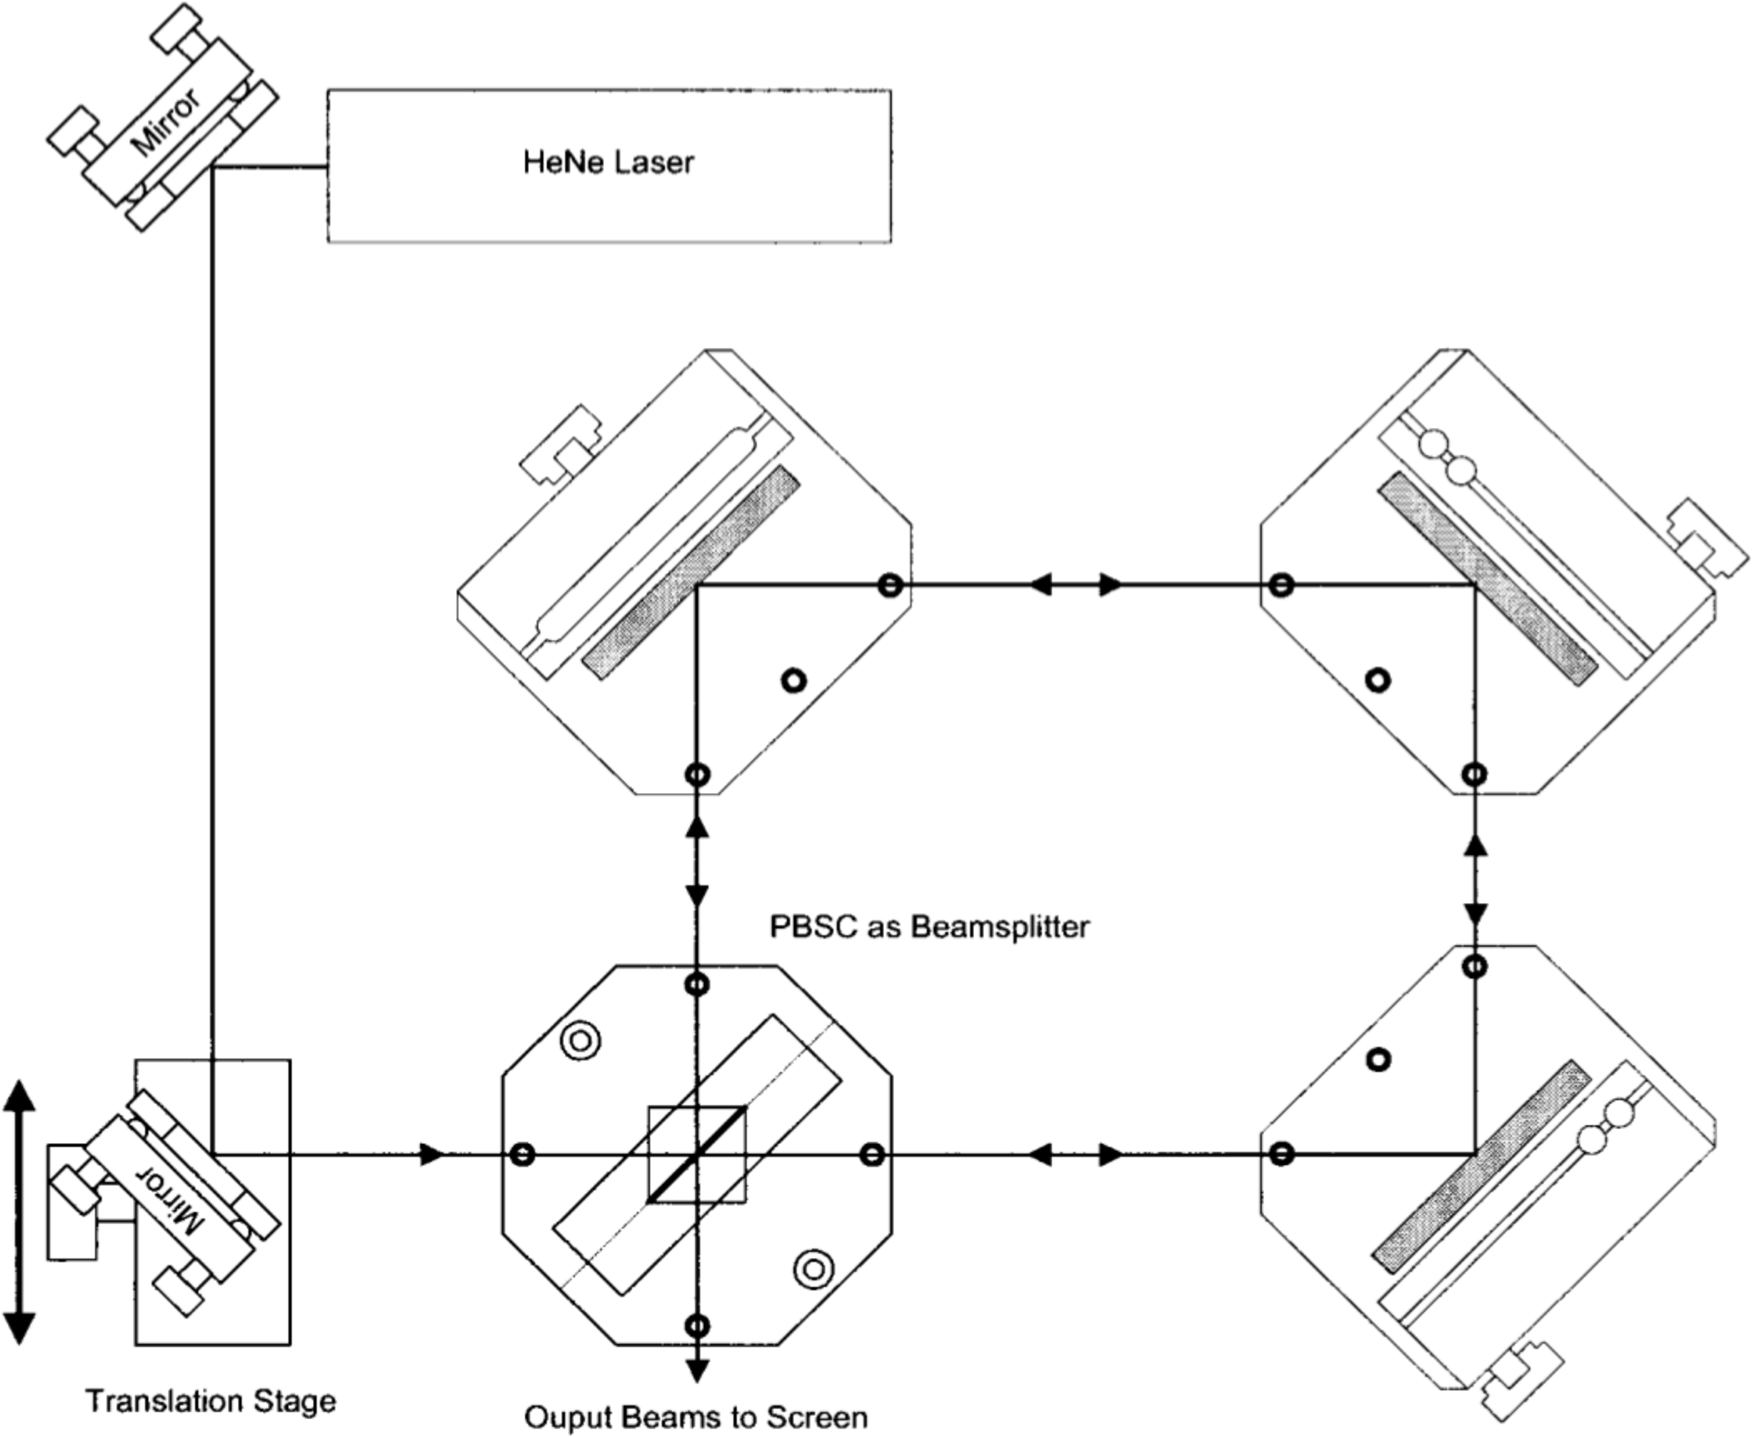
\includegraphics[width=\linewidth]{./figures/aufbau.pdf}
\caption{The Sagnac Interferometer}
\label{fig:interferometer}
\end{figure}
If the interferometer is perfectly adjusted, the resulting beams will overlap at all stages of the interferometer. To manipulate each beam individually, it is necessary to separate their superposition. To do so the laser, or in this case the mirror between the laser and the second mirror, has to be moved in the direction that is shown by the arrow in the picture. This results in the two beams following different paths after entering the PBSC. During this stage, one of the beams can be sent through a medium, making it possible to measure the medium's refraction index.\\

\subsection{Interference}
\label{sec:Interference}
For interference to happen, the linearly polarised beam emitted by the HeNe laser is split by a polarising beam splitter cube (PBSC). The coordinate system is chosen at the PBSC so that the beam hitting the cube is moving in the $z$-direction, with the $x$-coordinate lying in the experiment's optical plane. The laser is positioned in such a way that its linear polarisation lies in the optical plane.\\
Before the beam enters the PBSC, it moves through a polarisation filter. The filter's rotation angle is posed to match the traditional polar angle $\phi$ in the $x y$-plane.\\
This way, the beam leaving the polariser has the electric field
\begin{align}
  \label{eq:E_pbsc}
  \vec{E}_\text{PBSC} &= \frac{E_0}{\sqrt{2}} \cos\left(kz - \omega t\right) \left( \cos(\phi)\vec{e}_x + \sin(\phi) \vec{e}_y \right)
\end{align}
with the rotation angle of the polariser $\phi$.\\
The next step is the splitting of the beam, after which one of the partial beams goes through a phase-shift before reuniting them.\\
Inducing a phase shift $\delta$ in a beam is achieved by application of the translation operator 
\begin{align}
  \hat T(\delta) \coloneqq \exp\left(\frac{\delta}{\omega} \partial_t\right) \tp
\end{align}
But the PBSC does not only split the beam, but also splits its polarisations. In this experiment, the PBSC is positioned in a $\frac{\pi}{4}$ angle to the incoming beam, so that the intensities of the transmitted and that of the reflected polarisation are the same. For simplicity, the incoming beam's linear polarisation will be taken to have $\delta = \frac{\pi}{4}$, because this way, the $x$- and $y$-components have the same amplitude of $\frac{E_0}{\sqrt{2}}$. Due to the PBSC's tilt, the spllitting surface is aligned with the beam's $y$-component. This way, the $y$-component is transmitted, while the $x$-component undergoes reflection and phase-shift, which is why the full aperture from the PBSC to the interferometer's end also has to project the $x$- and $y$-components accordingly. For this, the parity operators 
\begin{align}
  \hat{P}_L &=
  \begin{pmatrix}
      0 & 0 \\
      0 & 1 
  \end{pmatrix} \\
  \hat{P}_R &=
  \begin{pmatrix}
      1 & 0 \\
      0 & 0 
  \end{pmatrix}
\end{align}
are very useful. Using these, the combined projection and translation operator representing the aperture from PBSC to the leaving point of the interferometer can be written as 
\begin{align}
  \hat{T}_\text{Int}(\delta) \coloneqq \left(\hat T(0)\hat{P}_L + \hat T(\delta)\hat{P}_R\right) \tp
\end{align}
At this point, the requirement for the monochromaticity of the light used in interference experiments becomes manifest: The translation operator directly depends on the frequency $\omega$ (and therefore on the wavelength $\lambda$). For this reason multichromatic light would get a different phase shift for each colour, which would smear the interference pattern the further it derives from monochromaticity.\\
Applying this translation operator on the electric field in \autoref{eq:E_pbsc} yields the split electric field 
\begin{align}
  \vec{E}_\text{Int} &= \hat{T}_\text{Int}(\phi) E_\text{PBSC} &= \frac{E_0}{\sqrt{2}} \left( \cos\left(kz - \omega t\right) \cos(\phi)\vec{e}_x + \cos\left(kz - \omega t + \delta\right) \sin(\phi) \vec{e}_y \right) \tp
\end{align}
Now, there is only one thing that prohibits the two partial beams from interfering with each other: The fact that their polarisations are perpendicular to each other. To fix this, a final polarisation filter is placed in the reunited beams' path, at an angle of $\frac{\pi}{4}$. This reduces the respective amplitudes by a factor of $\odiv{\sqrt{2}}$. The final electric field is 
\begin{align}
  \vec{E} &= \frac{E_0}{2} \left( \vec{e}_x + \vec{e}_y \right) \left( \cos\left(kz - \omega t\right) \cos(\phi) + \cos\left(kz - \omega t + \delta\right) \sin(\phi) \right) \tp
\end{align}
To get the intensity from this, the equation 
\begin{align}
  I &\propto \langle \hspace{1mm} |\vec{E}|^2\rangle_t
\end{align}
with them time average operator $\langle\text{F}\rangle_t \coloneqq \frac{1}{T}\int_0^T dt F$ performing a time-integral over one period (here: $T = 2\pi$) is used.\\
Computing this for the given case, the intensity becomes
\begin{align}
  I &\propto \langle \hspace{1mm} |\cos\left(kz - \omega t\right) \cos(\phi) + \cos\left(kz - \omega t + \delta\right) \sin(\phi) |^2\rangle_t \tp
\end{align}
The absolutes do not have any influence, as their argument is real and the square makes them obsolete. Therefore, using the fact that 
\begin{align}
  \langle \cos^2(\omega t + K)\rangle_t = \oh
\end{align}
and \begin{align}
  \langle \cos(\omega t + K)\cos(\omega t + K + \delta)\rangle_t = \cos{\delta}
\end{align}
for any $K$, the intensity becomes 
\begin{align}
  I \propto 1 + 2 \cos(\phi)\sin(\phi) \cos(\delta) \tp
\end{align}
From this it follows that constructive interference happens at $\delta = 0$, while destructive interference happens at $\delta = \pi$, so the minimum/maximum intensity is 
\begin{align}
  I_\text{min/max} \propto 1 \pm 2 \cos(\phi)\sin(\phi) \tp
\end{align}


\subsection{The Contrast}
An important quantity for interferometers is the contrast. The name is self-explanatory: Just like in the case of colours, where the contrast between two colours is highest if they are opposite to each other (for example black and white) and lowest if both colours are the same, the contrast in an interference picture is defined as 
\begin{align}
  K &\coloneqq \frac{I_\text{max}-I_\text{min}}{I_\text{max} + I_\text{min}} \tc
  \label{eq:contrast}
\end{align}
with minimal and maximal intensities $I_\text{min}$ and $I_\text{max}$.\\
The closer the contrast is to $1$, the better it is. On the other hand, it is worse the lower it is. The ideal contrast therefore occurs for $I_\text{min}=0$, while the worst case is that there are no minima/maxima, meaning that $I_\text{min}=I_\text{max}$.\\
In this experiment, the contrast will be measured dependent on the phase angle of a polarisation filter that has been positioned in the beam's path. For this, the contrast takes the form 
\begin{align}
  \label{eq:contrast}
K &= \sin(2\phi) \tp
\end{align}
This is a result from the considerations in \autoref{sec:Interference} and can be rescaled by a factor $K_0 \in [0,1]$ to account for physical effects that reduce the contrast, like imperfect polarisation overlap, reduced coherence, etc.


\subsection{The Refraction Index}
The refraction index of a medium is a measure for how fast light travels inside that medium. It is manifest in the dispersion relation inside the medium, effectively scaling the speed of light's vacuum value. This means that 
\begin{aquation}
  n &= \frac{c_\text{vac}}{c_\text{med}} \tp 
\end{aquation}
Plugging this into the vacuum dispersion relation, the resulting refraction index inside the medium, depending on the wave number inside the medium, is
\begin{aquation}
  n &= \frac{\lambda_\text{vac} k}{2\pi} \tp
\end{aquation}
In any medium with refractive index $n$, the phase shift that occurs when a beam has moved a distance $L$ is 
\begin{aquation}
  \varphi &= \frac{2\pi}{\lambda} n L \tp
\end{aquation}


\subsection{Solid Medium}
Now first consider the case of the aforementioned rotation holder holding only one glass plate, with the second beam going through air with $n \approx 1$. This case is shown in \autoref{fig:glasplaettchen}. The phase shift then is 
\begin{align}
  \Delta \delta\brr{\theta} &= \frac{2\pi L}{\lambda_\text{vac}} \left(\frac{n-1}{2 n} \theta^2 + \mathcal{O}\brr{\theta^4}\right) \tp
\end{align}
For two glass plates that are tilted wrt each other at an angle of $20\text{°}$, the phase shift takes a different form. Taking the angle $\theta \rightarrow \theta \pm \theta_0$ for the two cases (with $\theta_0 = 10 \text{°}$) yields the two phase shifts
\begin{align}
  \Delta \delta_\pm\brr{\theta} &= \frac{2\pi L}{\lambda_\text{vac}} \left(\frac{n-1}{2 n} \brr{\theta \pm \theta_0}^2 + \mathcal{O}\brr{\theta^4} \right) \tp
\end{align}
To get the total phase shift for two plates, these two have to be summed over to get
\begin{align}
  \label{eq:delta_tot}
  \Delta \delta_\text{tot}\brr{\theta} &= \frac{2\pi L}{\lambda_\text{vac}} \left(\frac{n-1}{2 n} \brr{\theta^2 + \theta_0^2} + \mathcal{O}\brr{\theta^4} \right) \tp
\end{align}

This quantity is the phase shift that is achieved when rotating the rotation holder over the angle $\theta$. It can exceed $2\pi$. Since the interference pattern measured by the photo diode is $2\pi$ periodic, it is possible that multiple maxima occur during this rotation. The number of maxima is 
\begin{align}
  \label{eq:number_of_maxima}
  M &= \frac{\Delta \varphi}{2\pi} \tp
\end{align}

% \begin{figure}
%   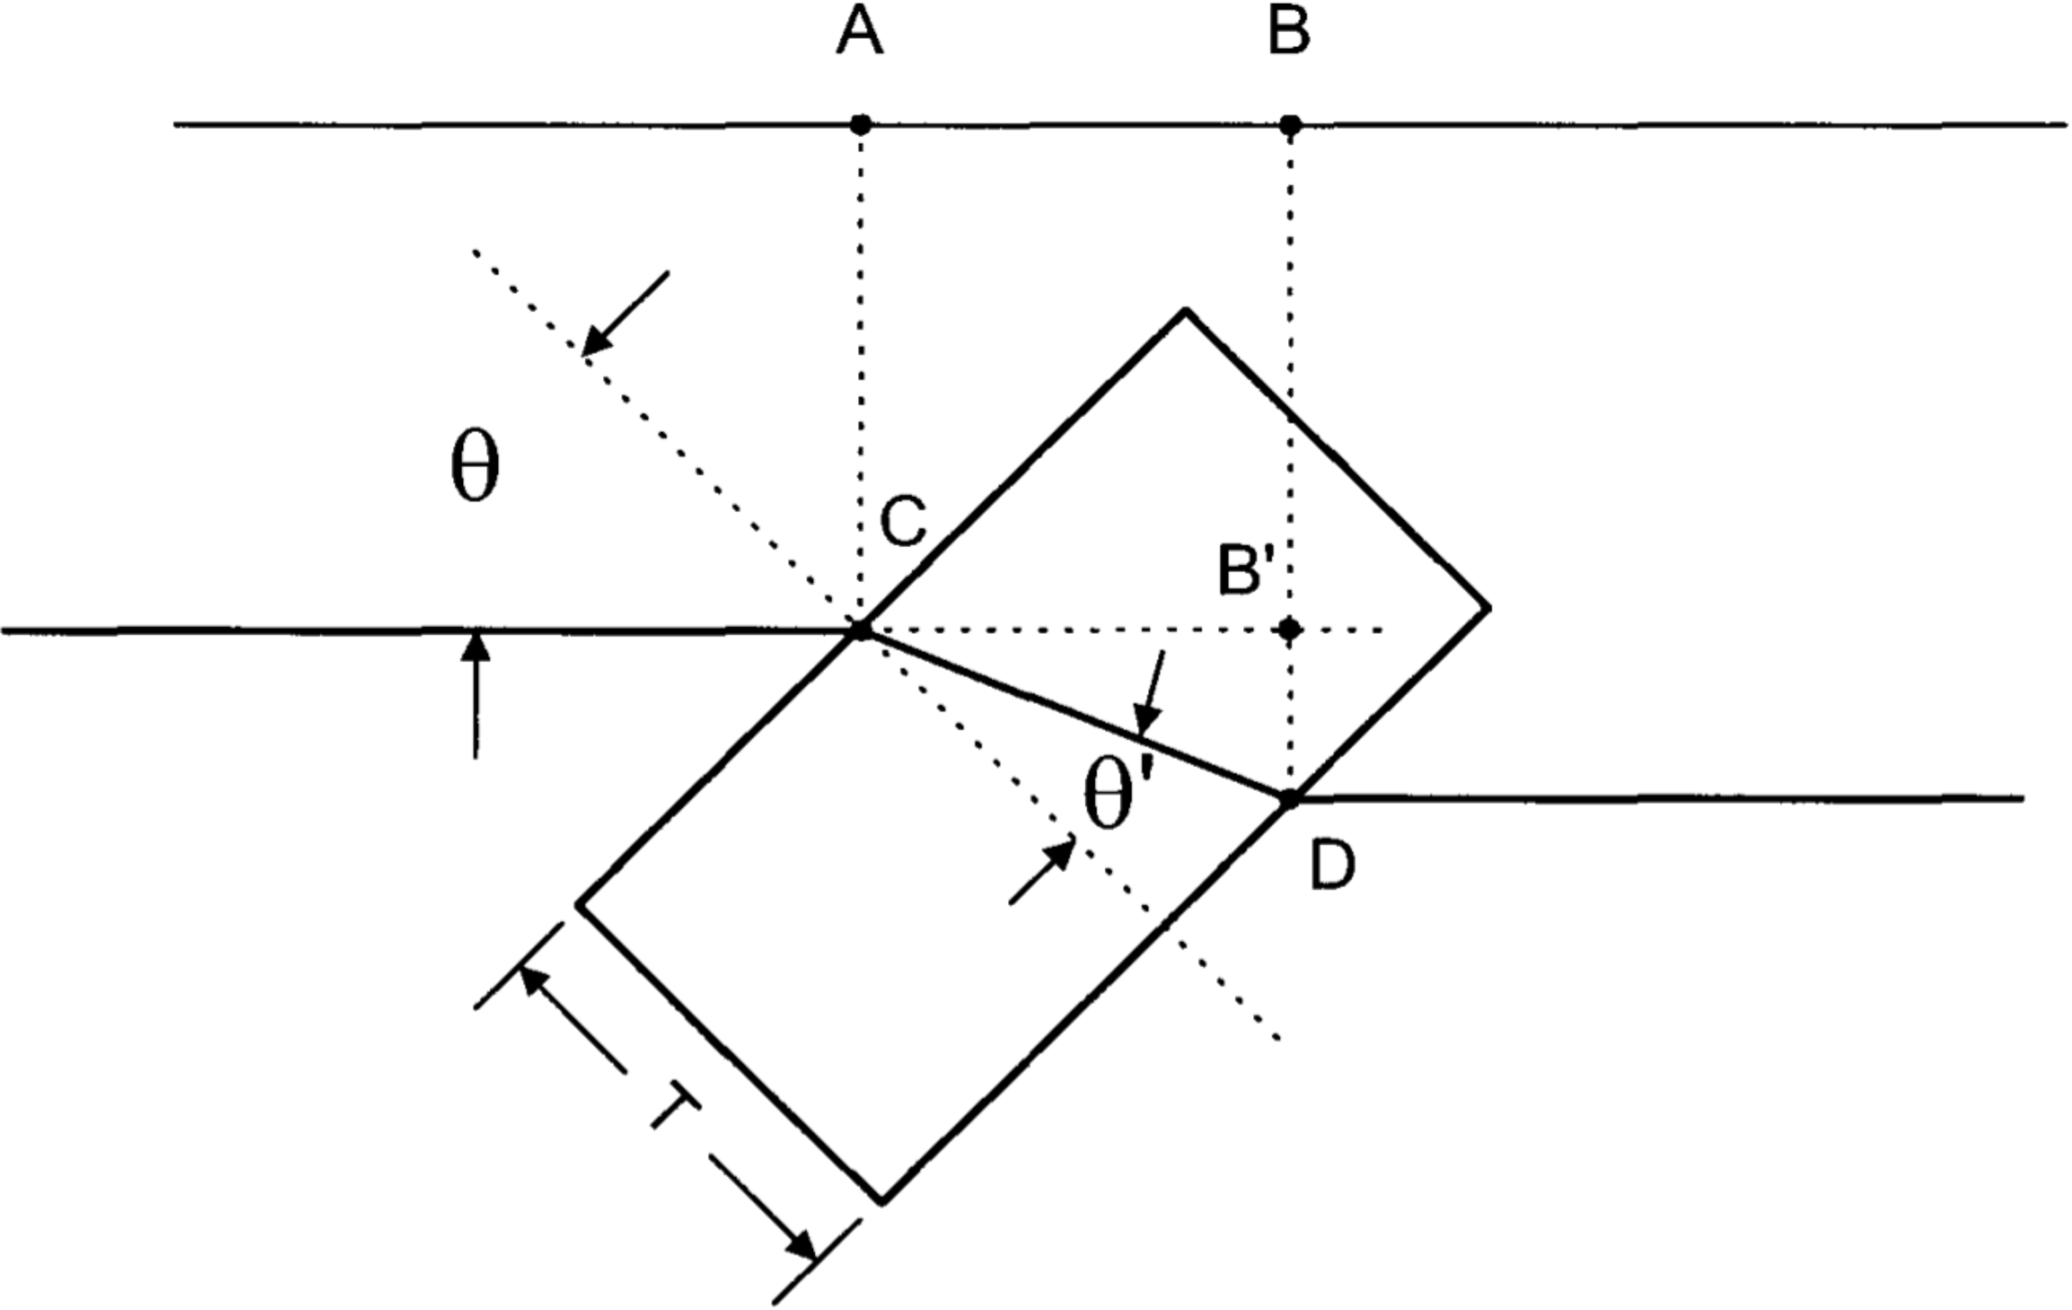
\includegraphics[width=\linewidth]{./figures/glasplaettchen.pdf}
%   \caption{The glass plate}
%   \label{fig:glasplaettchen}
% \end{figure}

% Both beams will have such a phase shift after moving through the distance $L$, and the phase shift will be different since the media are different. But their relative phase shift is just the difference between the total phases. For this reason, the phase shift caused by one beam traveling through a medium of length $L$ while the other travels through a medium with $n \approx 1$ (like the vacuum or air) will be 
% \begin{aquation}
%   \label{eq:phase_shift}
%   \varphi &= \frac{2\pi}{\lambda} (n - 1) L \tp
% \end{aquation}
% The number of interference maxima that occurs due to a phase shift is 
% \begin{aquation}
%   N &= \frac{\varphi}{2\pi} \tp
% \end{aquation}
% Plugging \autoref{eq:phase_shift} into this equation yields 
% \begin{aquation}
%   n &= 1 + \frac{N\lambda}{L} \tc
% \end{aquation}
% which makes it possible to determine the refractive index when $L$, $\lambda$ and $N$ are known.

\subsection{Gaseous Medium}
To measure this index, one of the beam is lead through a gas cell. The difference in the speed of light inside the cell yields a phase difference 
\begin{aquation}
  \Delta \varphi &= \frac{2 \pi L}{\lambda_\text{vac}}\left(n-1\right)
\end{aquation}
between the two beams, which results in them interfering with each other after being reunited. The number of maxima of interference is proportional to the phase difference. It is 
\begin{aquation}
  M &= \frac{\Delta \varphi}{2 \pi} \tp
  \label{eq:interference_maxima}
\end{aquation}
The refractive index is pressure and temperature dependent. To relate it to these quantities, the Lorentz-Lorenz equation 
\begin{aquation}
  \frac{n^2-1}{n^2+1} &= \frac{A p}{R T}
  \label{eq:Lorentz-Lorenz}
\end{aquation}
with pressure $p$, temperature $T$, gas constant $R$ and refractivity $A$.\\
Since the refraction index of air is $\approx 1$, it can be expanded, yielding
\begin{aquation}
  n &= \approx \sqrt{1 + \frac{3 A p}{R T}} \tp
\end{aquation}
This means that the refraction index can be measured by varying the gas's pressure and/or temperature.